% TODO(section): add archi section pointer
En esta sección se detallan las decisiones infraestructurales tomadas para llevar la arquitectura previamente mencionada y
abordada en la sección correspondiente a la práctica teniendo en cuenta el uso de recursos de las aplicaciones,
el presupuesto del equipo y las necesidades actuales, a su vez permitiendo el escalamiento y crecimiento del proyecto.

Por otro lado, se especifica el proceso de integración y despliegue de código de forma continua y por versiones,
como también las revisiones automatizadas de errores de código, inconsistencia de formatos y de filtrado de credenciales.

\subsubsection{CI/CD \& Workflows}

\begin{figure}[H]
\centering
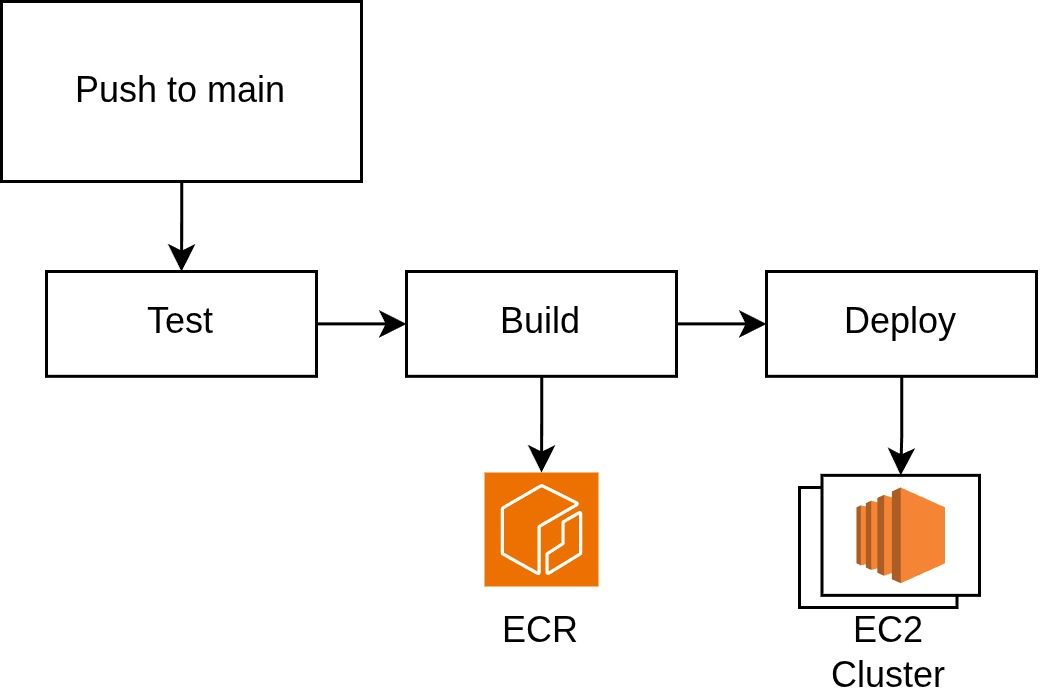
\includegraphics[width=0.5\textwidth]{img/08-implemented-solution/devops/core-workflow.jpg}
\caption{Visión general del 'workflow' de integración y despliegue continuo del \textit{core-service}.}
\end{figure}

\begin{figure}[H]
\centering
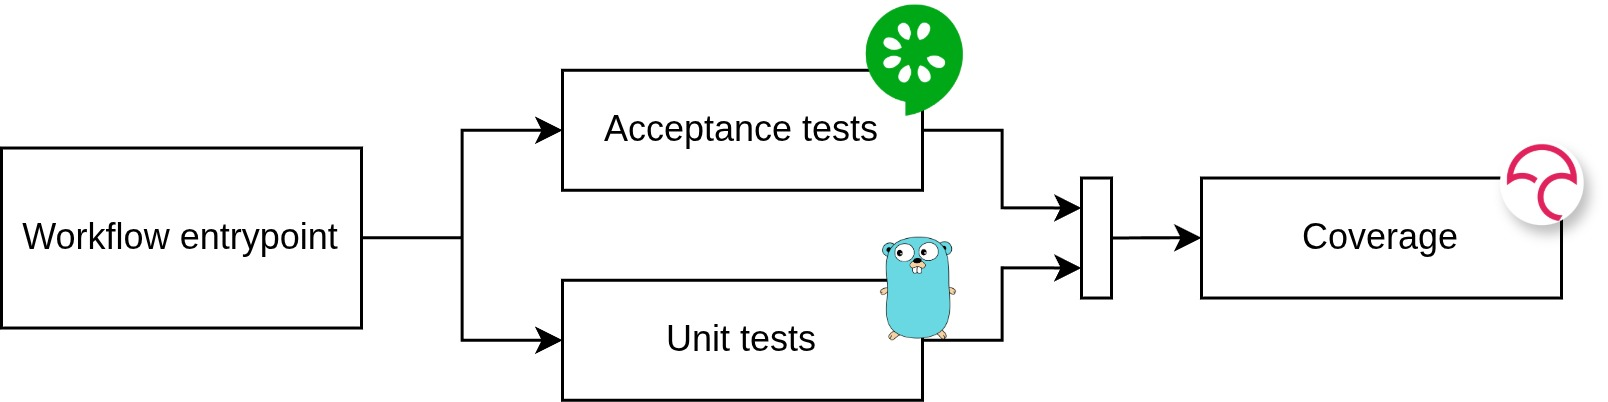
\includegraphics[width=0.75\textwidth]{img/08-implemented-solution/devops/test-pipeline.jpg}
\caption{Pipeline de ejecución de Tests.}
\end{figure}

\begin{figure}[H]
\centering
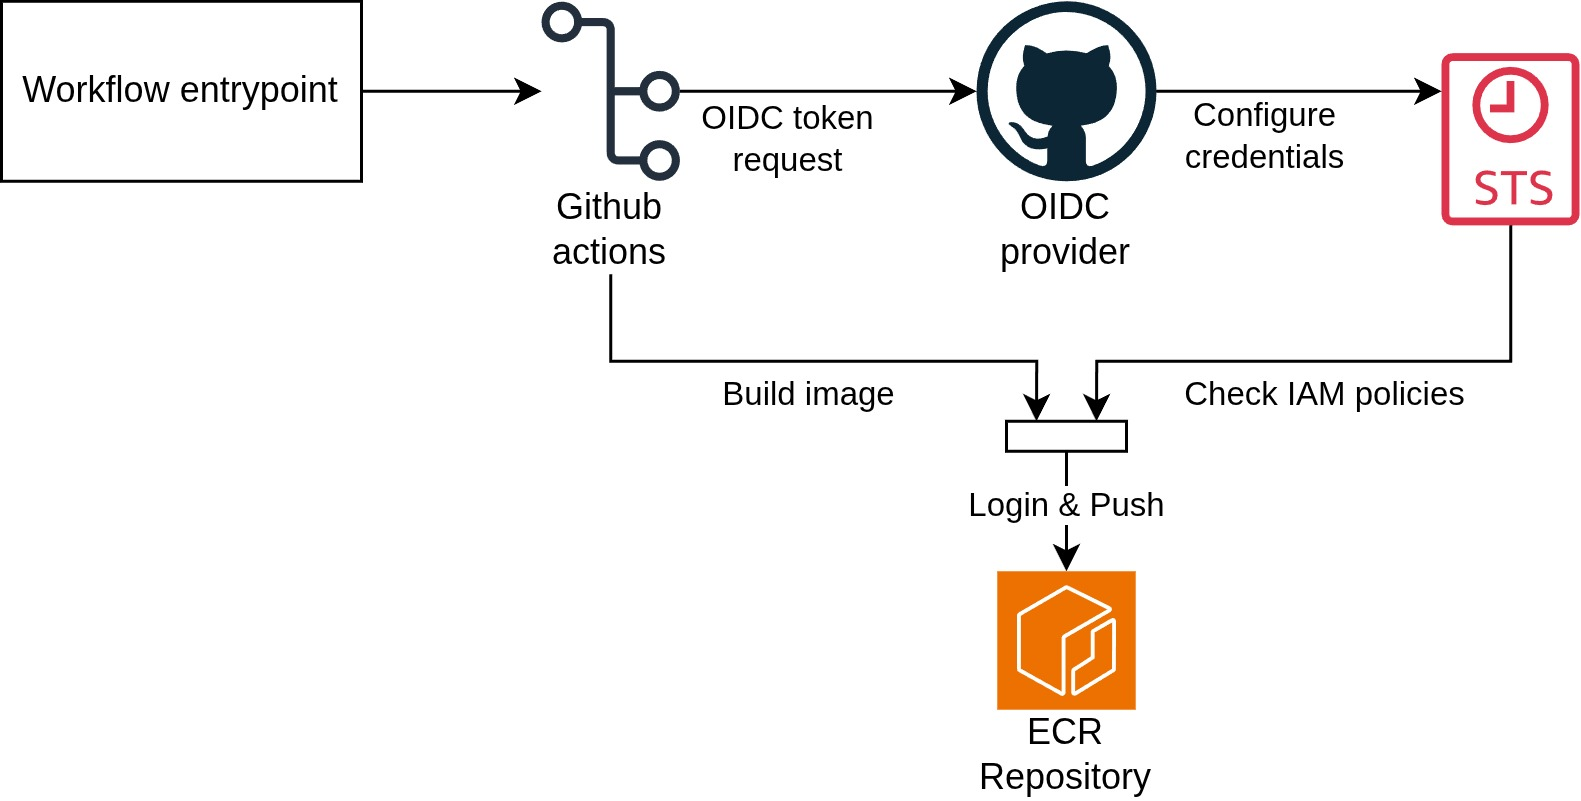
\includegraphics[width=0.75\textwidth]{img/08-implemented-solution/devops/build-pipeline.jpg}
\caption{Pipeline de construcción de la imagen de docker y subida a ECR.}
\end{figure}

\begin{figure}[H]
\centering
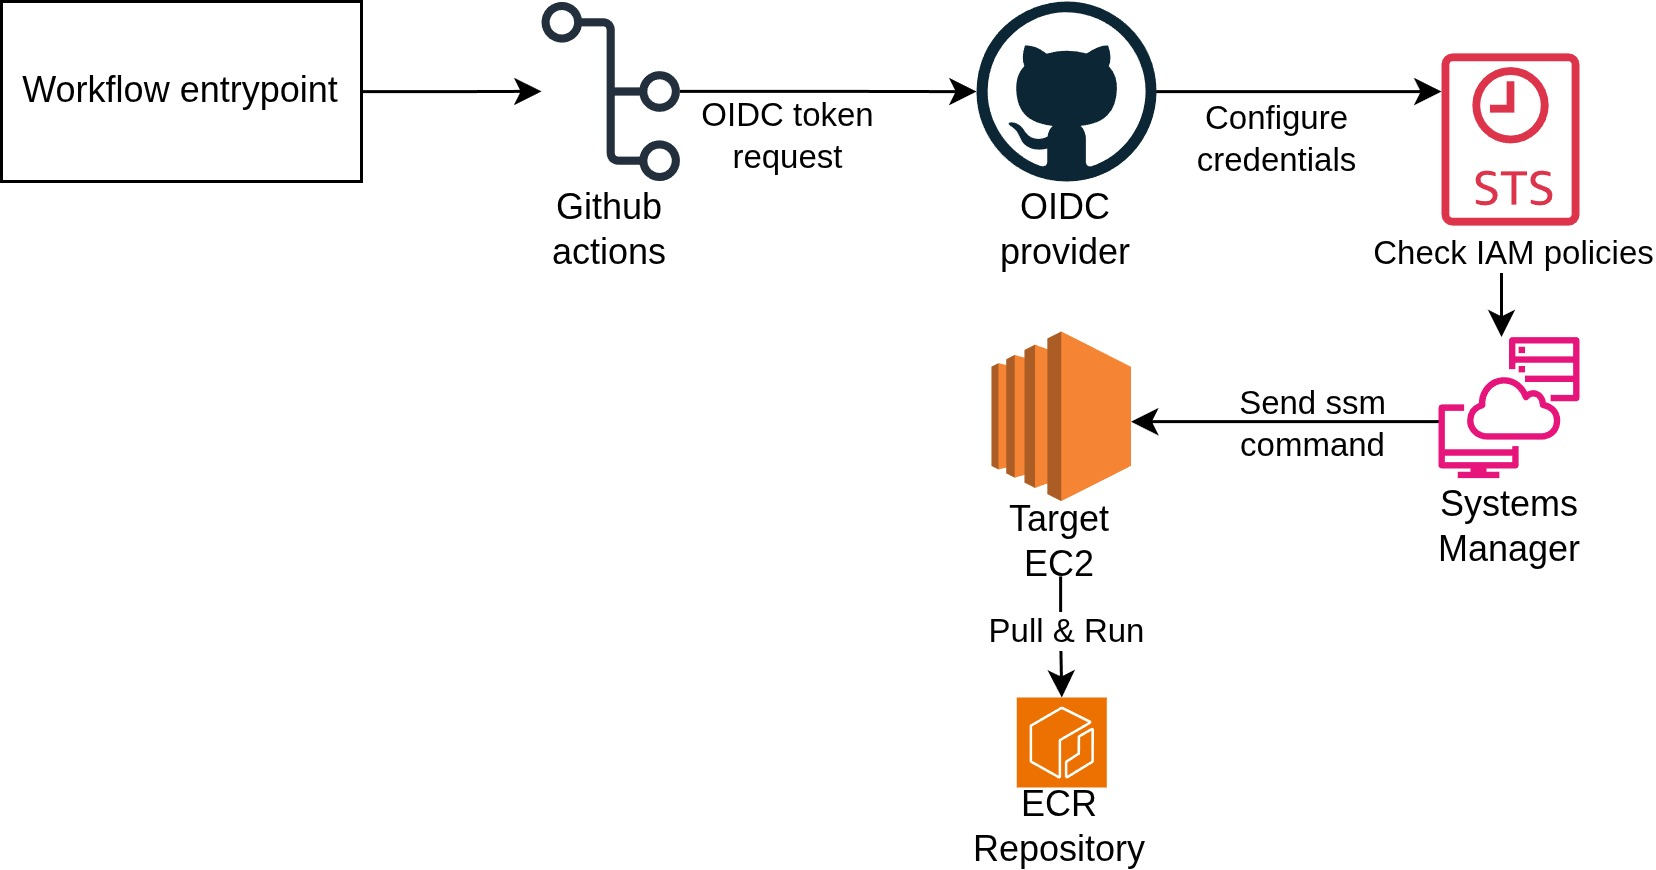
\includegraphics[width=0.8\textwidth]{img/08-implemented-solution/devops/deploy-pipeline.jpg}
\caption{Pipeline de despliegue del contenedor y ejecución en EC2.}
\end{figure}

\begin{figure}[H]
\centering
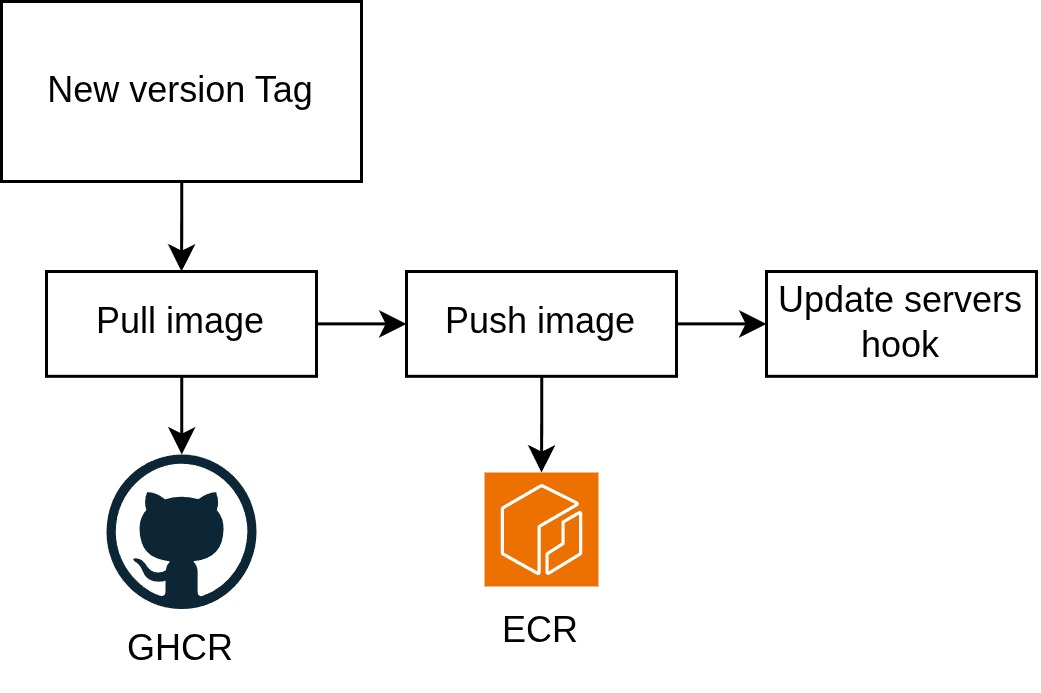
\includegraphics[width=0.5\textwidth]{img/08-implemented-solution/devops/server-workflow.jpg}
\caption{Visión general del 'workflow' de actualización de la imagen de los \textit{ftr-server}.}
\end{figure}

\subsubsection{Infraestructura}
INFRASTRUCTURE HERE

\begin{figure}[H]
\centering
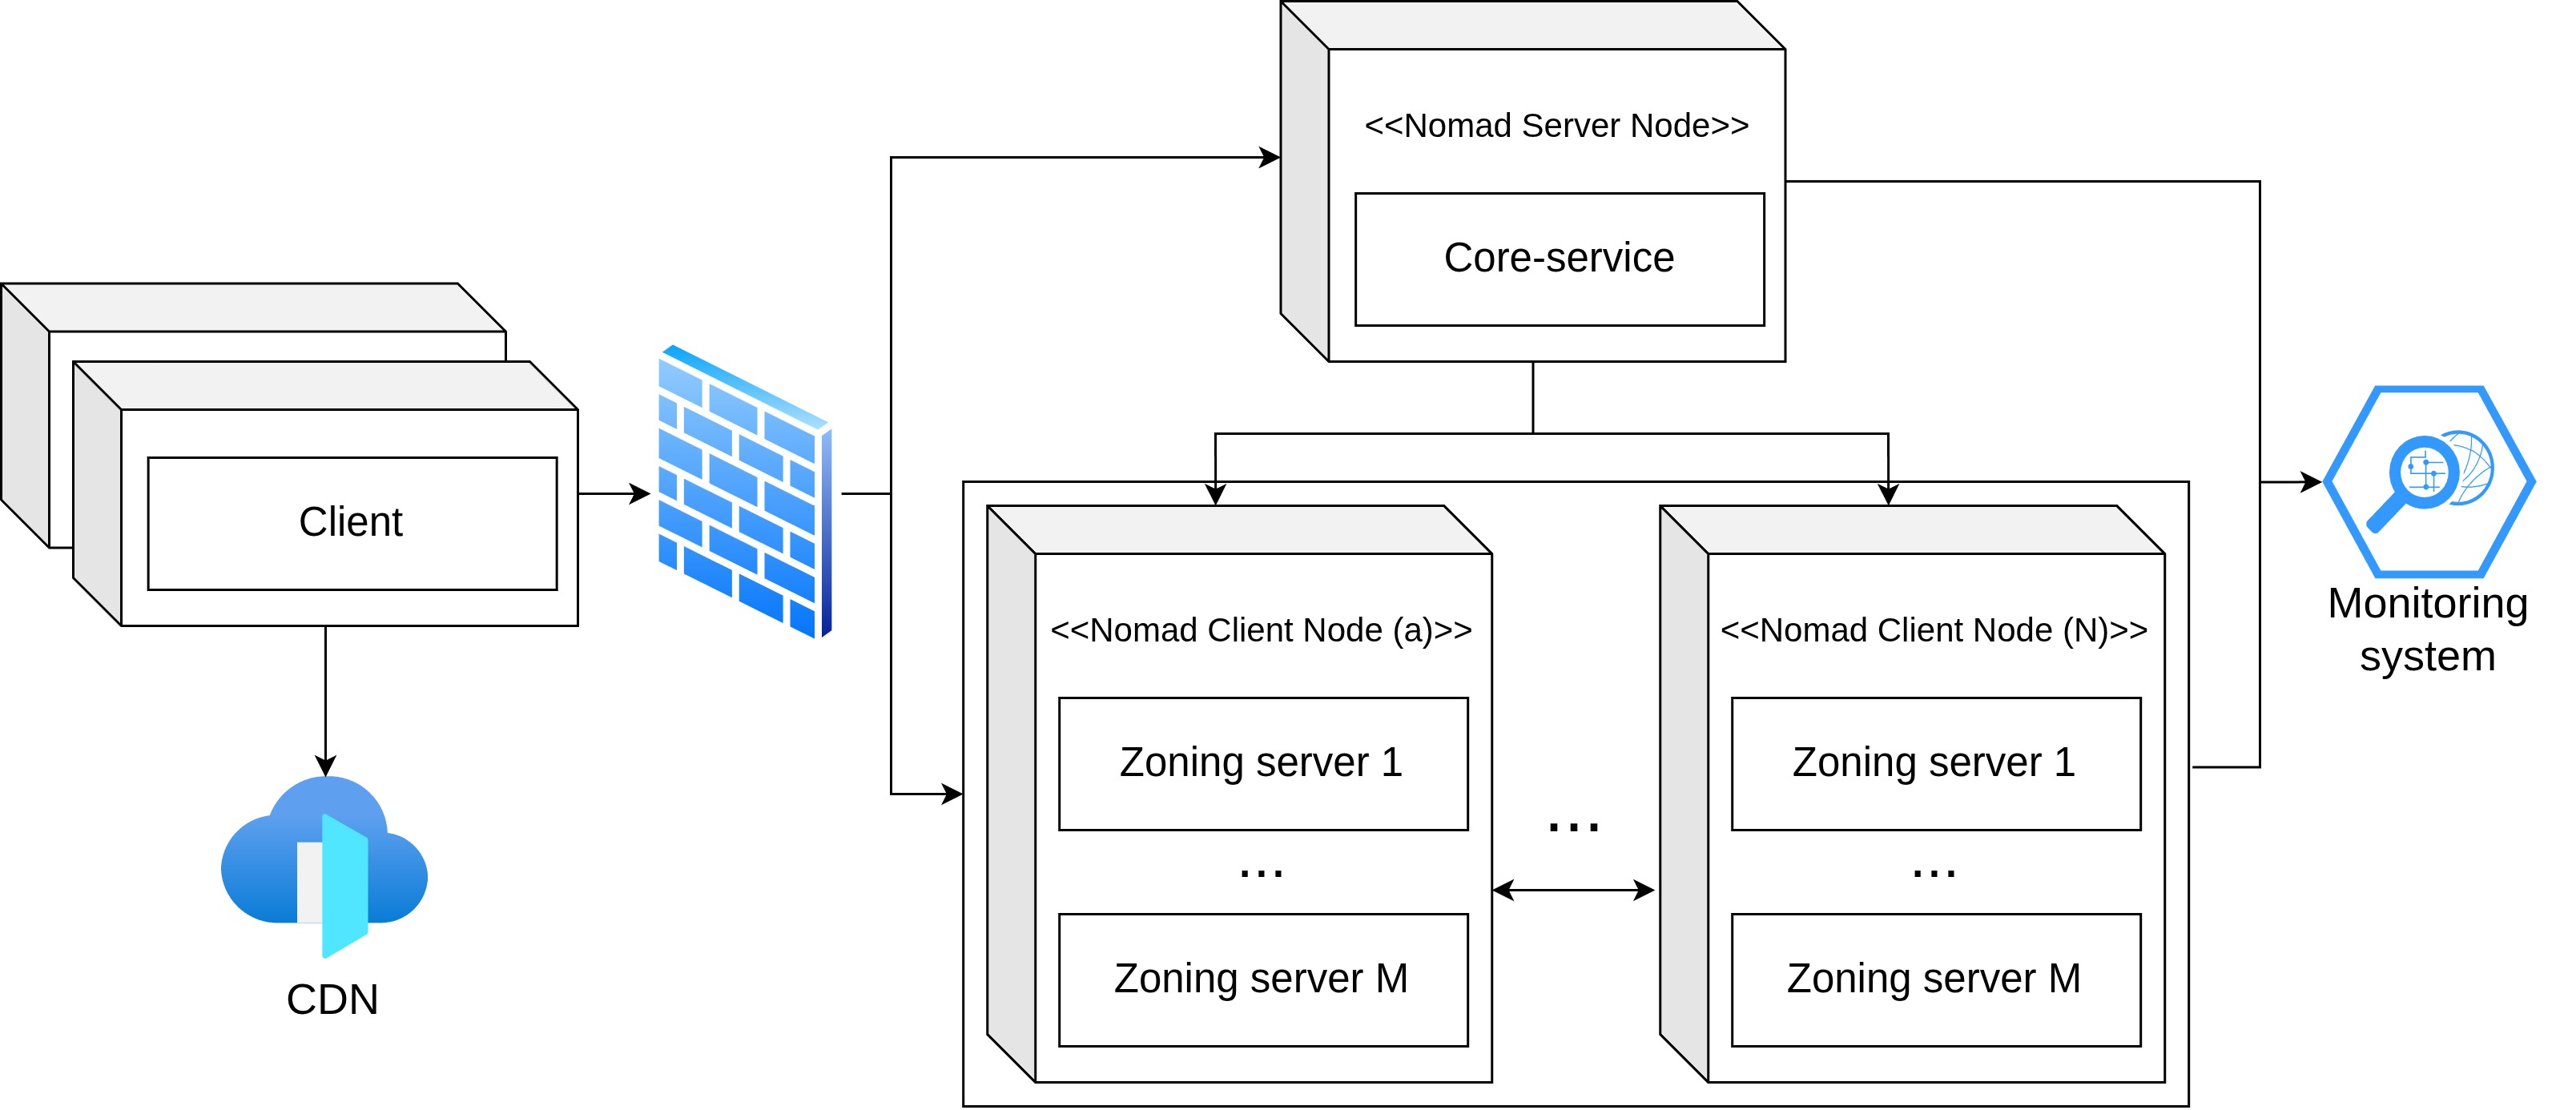
\includegraphics[width=1\textwidth]{img/08-implemented-solution/devops/deployment.jpg}
\caption{Product Vision de Feed the Realm.}
\end{figure}

\begin{figure}[H]
\centering
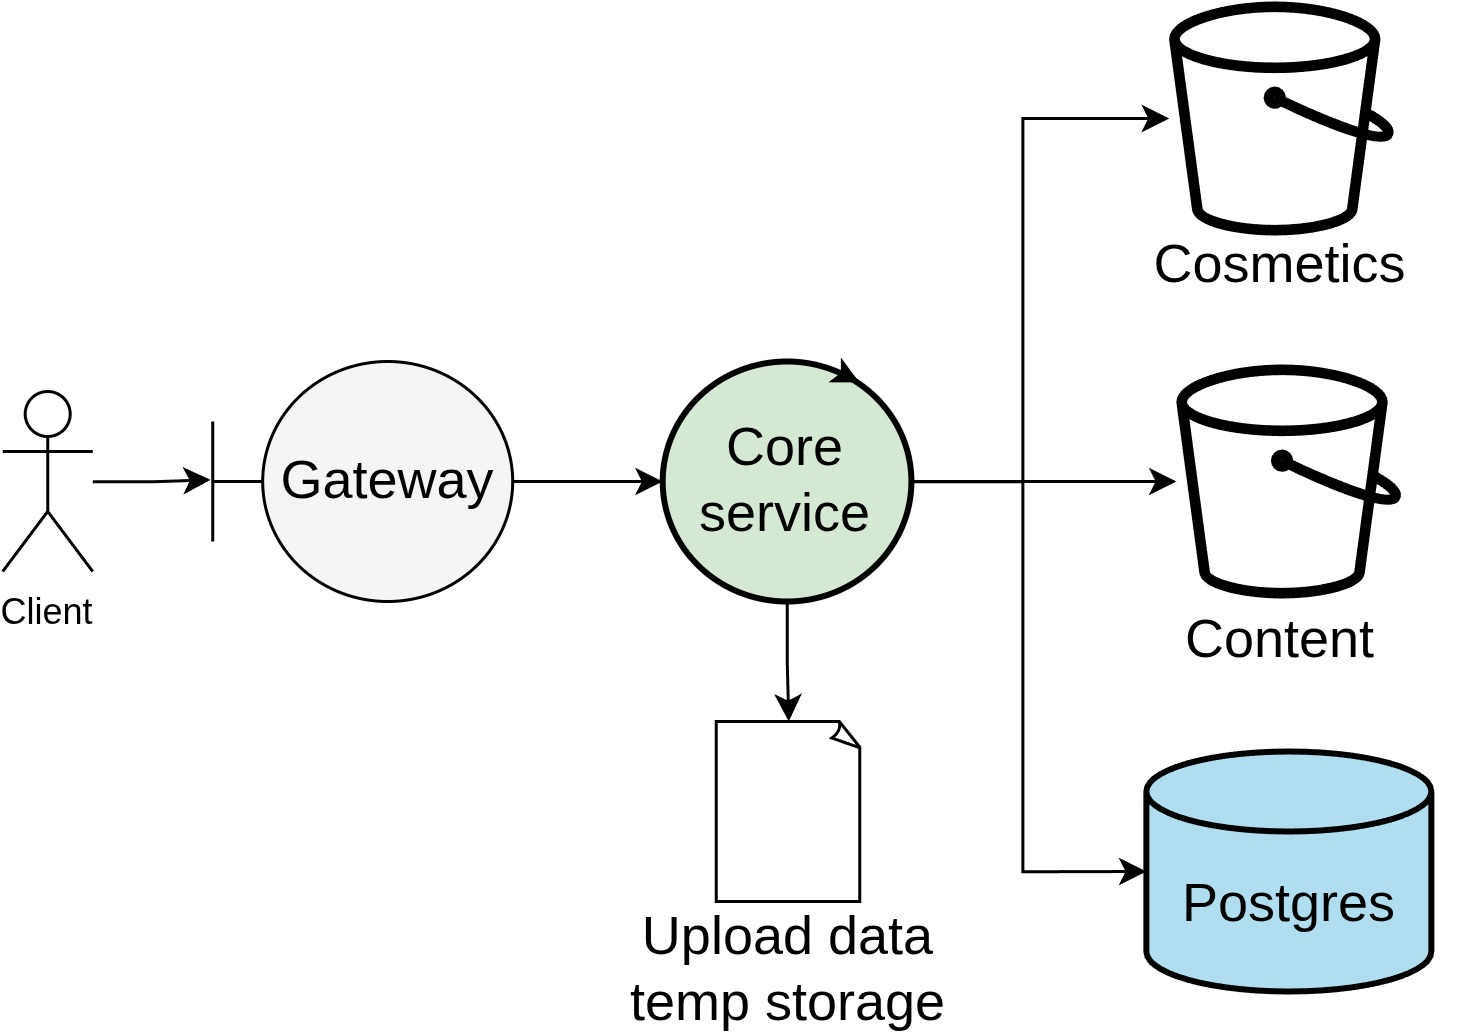
\includegraphics[width=0.5\textwidth]{img/08-implemented-solution/devops/core-robust.jpg}
\caption{Product Vision de Feed the Realm.}
\end{figure}

\begin{figure}[H]
\centering
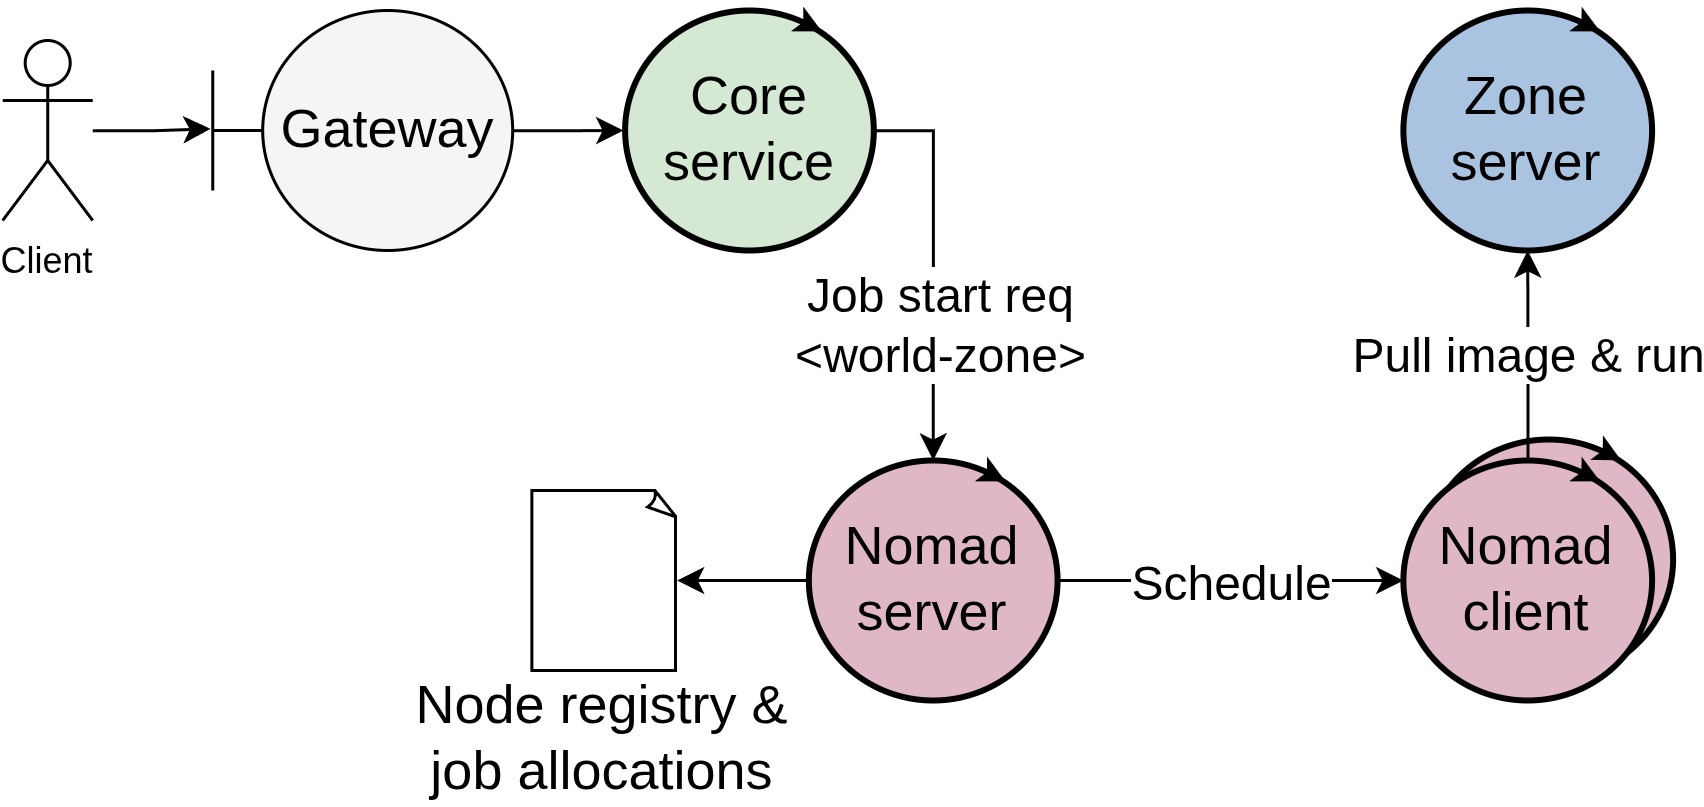
\includegraphics[width=0.6\textwidth]{img/08-implemented-solution/devops/nomad-robust.jpg}
\caption{Product Vision de Feed the Realm.}
\end{figure}

\begin{figure}[H]
\centering
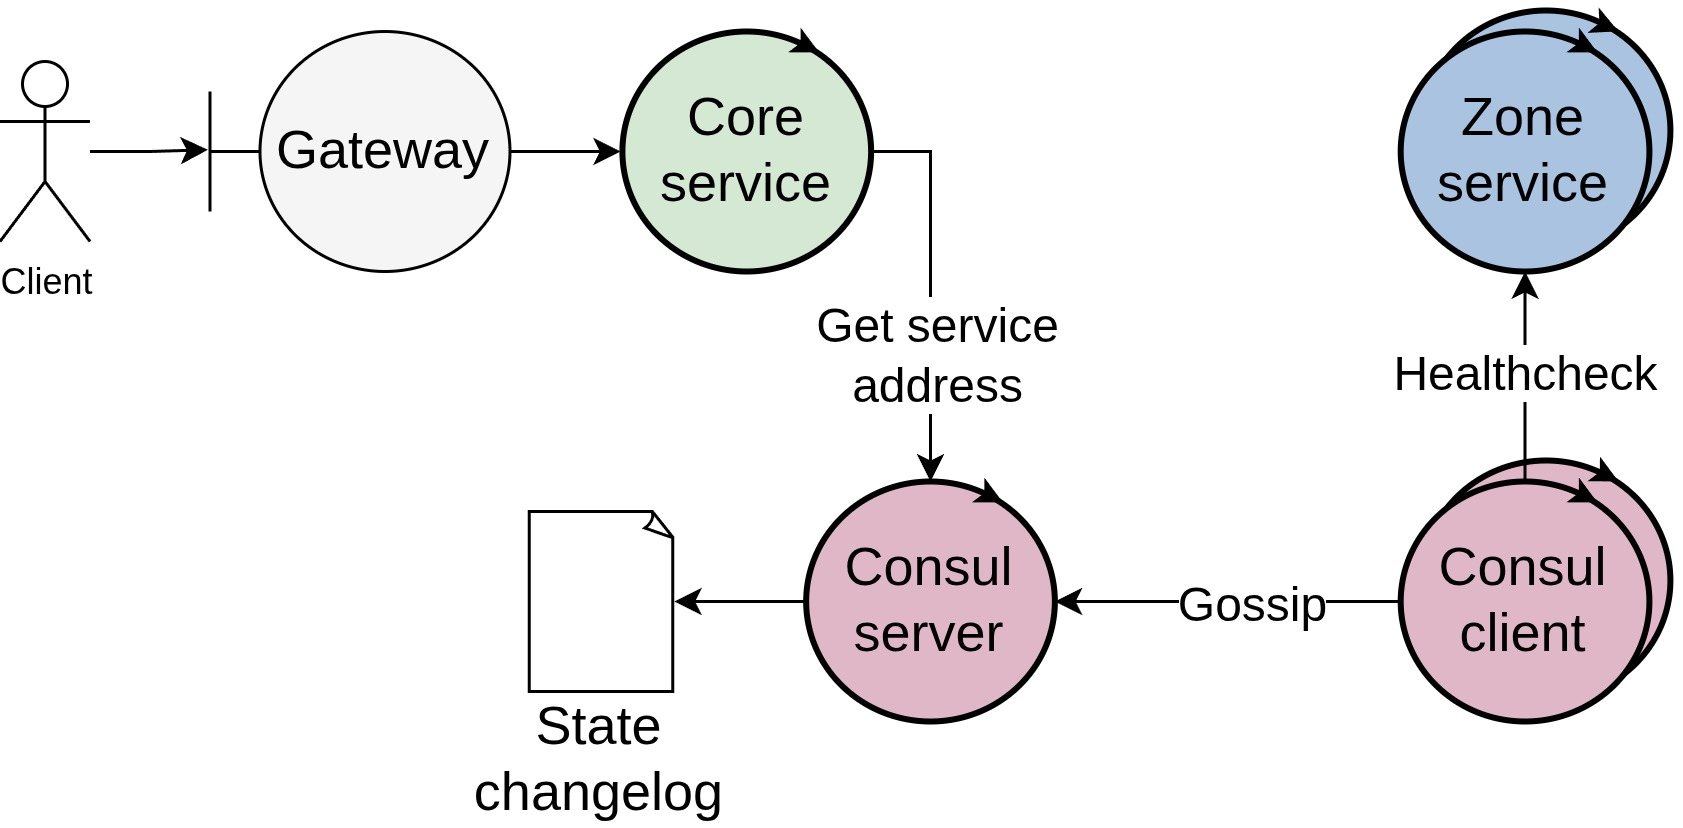
\includegraphics[width=0.6\textwidth]{img/08-implemented-solution/devops/consul-robust.jpg}
\caption{Product Vision de Feed the Realm.}
\end{figure}

\begin{figure}[H]
\centering
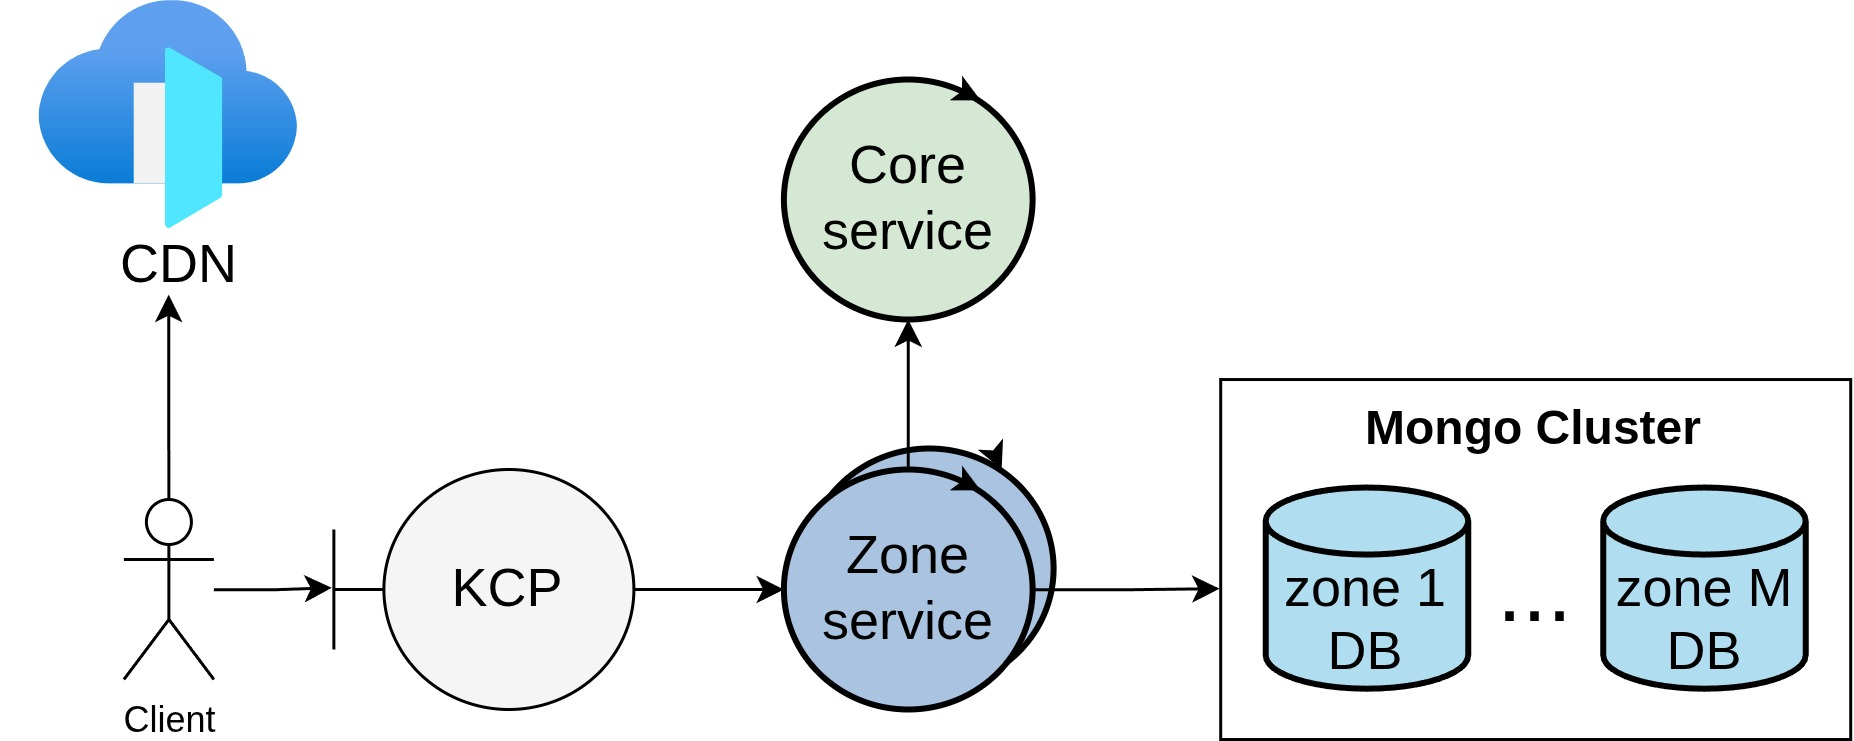
\includegraphics[width=0.65\textwidth]{img/08-implemented-solution/devops/game-robust.jpg}
\caption{Product Vision de Feed the Realm.}
\end{figure}

\subsubsection{Actualización de las aplicaciones 'Cliente'}
